\chapter{Algoritmi otkrivanja društvenih zajednica}

Ključan dio u pronalasku društvenih zajednica u društvenim mrežama su algoritmi koji ih otkrivaju. Oni moraju biti pouzdani i učinkoviti, ali se i izvršavati u prihvatljivom vremenskom okviru. Algoritmi se testiraju na brojnim skupovima podataka uz prikladne evaluacijske mjere kako bi se zaključilo u kojim uvjetima koji algoritam daje najbolje rješenje. 

Grafove koji predstavljaju društvene zajednice teško je prikazati u ravnini ako teže stvarnim veličinama koje se kreću u tisućama čvorova, a često i mnogo više, što znači da se ne može iz ljuske perspektive odrediti kako bi dobar raspored zajednica izgledao. To znači da su algoritmi koji pronalaze društvene zajednice nenadzirani algoritmi koji sami, bez primjera za učenje i unaprijednog znanja o njima pokušavaju pronaći rješenje. U društvenim mrežama algoritmi koriste topološke karakteristike i specifičnosti koje posjeduju ovakvi tipovi mreža. 

Dvije važne tehnike na kojima se temelji većina algoritama su particioniranje i grupiranje. Particioniranje grafova je proces u kojem se graf dijeli na unaprijed određeni broj manjih komponenti pomoću određenog svojstva. Svojstvo koje se može iskoristiti je minimalni rez. Ono se koristi tako da se graf podijeli na dva ili više razdvojenih podgrafova, a veličina reza koja se pokušava minimizirati je broj bridova koje je potrebno ukloniti da bi to ostvarili. Potrebno je odrediti i svojstvo koje bi odredilo veličinu komponenti kao primjerice minimalan ukupan stupanj vrhova kako bi se dobila rješenja koja imaju smisla. Zbog takvih zahtjeva ovakav pristup najčešće nije prihvatljiv jer broj zajednica nije moguće unaprijed odrediti.
Grupiranje je proces u kojem se entitete koji imaju zajedničke karakteristike svrstava u iste grupe. Pronalaženje grupa može dati informacije o skrivenim značajkama, vezama i svojstvima članova te koliko su međusobno čvrsto povezani. U hijerarhijskom grupiranju stvara se hijerarhija među zajednicama. Proces se može odvijati na dva načina, aglomerativni ili divizivni. U aglomerativnom načinu se koristi pristup koji ide od dna prema vrhu te se određeni čvor dodaje drugim sličnim čvorovima te se koristi određeni kriterij sličnosti. U divizivnom načinu veće grupe dijele se na manje uz korištenje određene mjere koja govori koliko je dobra trenutačna podjela prema kojoj će se odrediti konačan rezultat.



\section{Girvan-Newmanov algoritam}

Veliko zanimanje i rast aktivnosti znanstvene zajednice u području društvenih mreža potaknuo je rad Girvana i Newmana iz 2002. godine \cite{girvan2002community} u kojem su predstavili novi algoritam koji se po njima i naziva. Dotad poznati algoritmi pokušavali su pronalaženje zajednica riješiti tako da bi provodili hijerarhijsko grupiranje. U početnom koraku kreće se od nepovezanog grafa te se za svaki par vrhova računa težina koja predstavlja koliko su vrhovi bliski. Tada se bridovi se dodaju jedan po jedan počevši od onih vrhova čija je bliskost najveća. Postoji više načina kako izračunati bliskost i temelje se na broju puteva između čvorova, npr. broj vršno nezavisnih putova ili bridno nezavisnih putova i slično. Takve definicije ipak u nekim slučajevima nisu uspješne i daju krive rezultate. Događa se da se vrhovi koji su na rubovima zajednice, povezani jednim bridom prema ostatku mreže izdvajaju iz zajednice kojoj pripadaju i ostaju potpuno izolirani od svih zajednica. Girvan-Newmanov algoritam pokušava suprotno, pronaći bridove koji što manje doprinose povezanosti unutar zajednica. 

Algoritam traži bridove koji povezuju zajednice te ih kroz iteracije uklanja i izolira zajednice. Za pronalazak bridova koristi se mjera različitosti, u ovom slučaju mjera bridne centralnosti. Njezina vrijednost računa se za svaki brid tako što se za sve parove vrhova odredi najkraći put te se svim bridovima koji se nalaze u tom putu dodaje vrijednost 1. Ako postoji $N$ najkraćih putova između vrhova onda se u svim putevima svakom bridu vrijednost povećava za $ \dfrac{1}{N} $. Bridna centralnost svakog vrha na početku je postavljena na 0. Postupak se ponavlja dok god postoji bridova u grafu. Izračunavanje bridne centralnosti je skupa operacija jer je potrebno za svaki par vrhova u svakoj iteraciji pronaći najkraći put te odrediti bridne centralnosti Mora se provoditi u svakom koraku jer se inače mogu dogoditi pogreške u koracima algoritma zato što se mreža prilagođava novom stanju nakon uklanjanja svakog brida. Takva situacija može se dogoditi ako su dvije zajednice povezane sa više bridova. Tada je prema algoritmu, sigurno da će barem jedan od tih bridova imati visoku bridnu centralnost te se zato nakon njegovog uklanjanja vrijednost mjere mora ponovno odrediti, a onda će jedan od preostalih bridova imati najvišu vrijednost. Moguće je uštediti nešto resursa tako što se bridna centralnost izračunava samo za one vrhova na koje je uklanjanje prethodnog brida imalo utjecaja. 

\bigskip
\begin{algorithm}
\caption{Girvan-Newmanov algoritam}
\begin{algorithmic}[1]
	\STATE izračunati mjeru različitosti za sve bridove u grafu
	\STATE ukloniti brid sa najvećom vrijednosti mjere različitosti
	\STATE za svaki brid izračunati mjeru različitosti nakon uklanjanja brida
	\STATE ponavljati korake 2 i 3 dok ima bridova u grafu
\end{algorithmic}
\end{algorithm}
\bigskip

Konačno rješenje algoritma određuje se tako što se u svakoj iteraciji računa modularnost za trenutnu podjelu grafa. Modularnost je mjera koja se koristi za procjenu jakosti veza unutar zajednice i jakosti veza među zajednicama. Njome je moguće izmjeriti koliko je određena podjela grafa kvalitetna. Ona podjela koja ima najvišu vrijednost na kraju algoritma uzima se kao rezultat. O modularnosti i ostalim mjerama mjerenju rezultata više će biti rečeno u poglavlju \ref{vrednovanja_i_rezultati} koje se bavi vrednovanjem rezultata algoritama.


Postupak traženja zajednica tijekom rada algoritma može se predstaviti dendogramom. Dendogram je prema strukturi stablo gdje su listovi pojedini vrhovi mreže. Prema vrhu stabla vrhovi se spajaju u zajednice te konačno u cijelu strukturu grafa. Vrhovi povezani na nižim razinama imaju snažnije međusobne veze. Rez kroz stablo na bilo kojoj razini daje skup zajednica koji u tom trenutku postoji. Gdje stablo odrezati određuju se pomoću modularnosti. Primjer je prikazan na slici \ref{fig:dendogram}.

\begin{figure}
	%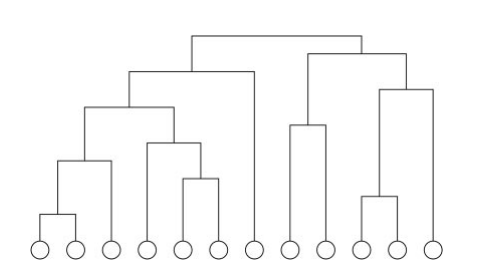
\includegraphics[width=\linewidth]{images/dendogram.png}
	\makebox[\textwidth][c]{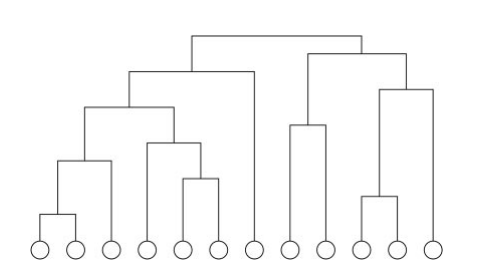
\includegraphics[width=0.8\textwidth]{images/dendogram.png}}
	\caption{Primjer hijerarhijskog stabla. Moguće je po koracima vidjeti kada je koji brid uklonjen iz mreže te kako su grupe nastale.}
	\label{fig:dendogram}
\end{figure}


\section{Louvaineov algoritam}